% Created 2024-08-04 Sun 14:44
% Intended LaTeX compiler: xelatex
\documentclass[a4paper,11pt,twoside]{article}
\usepackage{graphicx}
\usepackage{longtable}
\usepackage{wrapfig}
\usepackage{rotating}
\usepackage[normalem]{ulem}
\usepackage{amsmath}
\usepackage{amssymb}
\usepackage{capt-of}
\usepackage{hyperref}
\usepackage{libertine} \usepackage{amsmath}
\usepackage[width=200.00mm, height=240.00mm, left=3cm, right=3cm, top=3 cm, bottom=3cm]{geometry}
\usepackage{graphicx}
\graphicspath{ {./images/} }
\usepackage{multicol}
\author{Ryan P. Lynch}
\date{\today}
\title{Program 3B}
\hypersetup{
 pdfauthor={Ryan P. Lynch},
 pdftitle={Program 3B},
 pdfkeywords={},
 pdfsubject={},
 pdfcreator={Emacs 29.4 (Org mode 9.6.24)}, 
 pdflang={English}}
\usepackage{biblatex}

\begin{document}

\maketitle
\section*{Compiling \& Executed}
\label{sec:org427e9d9}
The screenshot below shows the compiling of the \emph{Kernel.java}, \emph{SyncQueue.java}, \emph{QueueNode.java} files and the execution of the Test2 class using the ThreadOS Shell.
\begin{center}
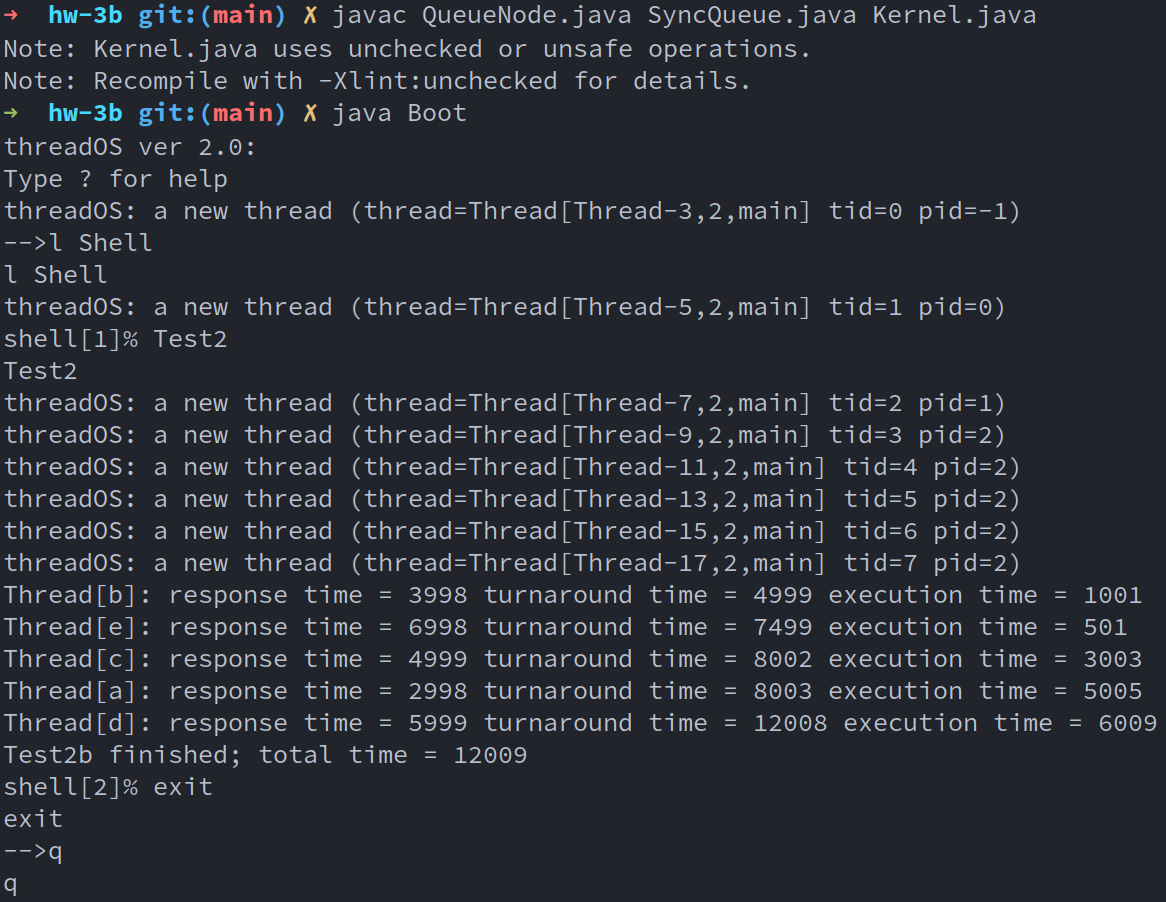
\includegraphics[width=.9\linewidth]{./Compile&Execution.png}
\end{center}
\end{document}
